\documentclass[10pt,a4paper]{article}
\usepackage[utf8]{inputenc}
\usepackage[T1]{fontenc}
\usepackage[a4paper,top=1.5cm,bottom=1.5cm,left=1.5cm,right=1.5cm]{geometry}
\usepackage{amsmath}
\usepackage{amssymb}
\usepackage{tikz}
\usetikzlibrary{calc,patterns}
\usepackage[dvipsnames,svgnames]{xcolor}
\usepackage{booktabs}
\usepackage{tabularx}
\usepackage{array}
\usepackage[bookmarks=false]{hyperref}

\title{Rubrik Nilai Tugas Minggu 2 : Pertidaksamaan Nilai Mutlak}
\author{Matematika untuk Sistem Informasi}
\date{}

\newenvironment{rubrik}{%
  \noindent
  \tabularx{\textwidth}{@{}>{\raggedright\arraybackslash}p{2.2cm}>{\raggedright\arraybackslash}X>{\centering\arraybackslash}p{1.1cm}>{\centering\arraybackslash}p{1.4cm}@{}}
  \toprule
  \textbf{Kriteria} & \textbf{Deskriptor} & \textbf{Maks} & \textbf{Skor} \\
  \midrule
}{%
  \bottomrule
  \endtabularx\par
}
\newcommand{\butir}[1]{\par\vspace{0.75em}\noindent\textbf{#1}\par\vspace{0.35em}}

\begin{document}
\maketitle

\noindent
Nama: \underline{\hspace{7.2cm}} \quad NIM: \underline{\hspace{4.2cm}}

\section*{Petunjuk penilai}
\begin{itemize}
  \item Tiap butir maksimum 100. Nilai tugas adalah rata-rata skor butir.
  \item Ketentuan skor:\par
  {\small
  \setlength{\tabcolsep}{4pt}%
  \begin{tabularx}{\linewidth}{@{}>{\raggedright\arraybackslash}p{2.1cm}>{\centering\arraybackslash}p{1.1cm}>{\raggedright\arraybackslash}X@{}}
  \toprule
  \textbf{Kriteria} & \textbf{Maks} & \textbf{Ketentuan} \\
  \midrule
  Langkah & 50 & Jika langkah terbaca dan tidak seluruhnya salah, skor minimal 25. Skor di bawah 25 hanya bila langkah salah total, tidak dimengerti, atau tidak terbaca. \\
  Jawaban & 30 & Harus ada dan benar. Skor hanya 0 atau nilai penuh. \\
  Penyajian & 20 & Harus ada dan benar. Skor hanya 0 atau nilai penuh. \\
  \bottomrule
  \end{tabularx}}
\end{itemize}

\butir{Butir 1. $|x + 2| < 1$ (100 poin)}
\begin{rubrik}
Langkah &
Satu sifat nilai mutlak diterapkan sampai diperoleh pertidaksamaan tanpa tanda mutlak, lalu diselesaikan. &
50 & \\
Jawaban &
$\mathrm{HP} = (-3, -1)$. &
30 & \\
Penyajian &
Garis bilangan: titik kosong di $-3$ dan $-1$, arsiran di antaranya.\par\vspace{0.4em}
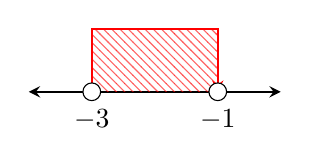
\begin{tikzpicture}[scale=0.8]
\draw[thick,stealth-stealth] (-4,0)--(0,0);
\draw[thick,-stealth,Red] (-3,0)--(-3,1)--(-1,1)--(-1,0);
\path[pattern=north west lines,opacity=.6,pattern color=Red] (-3,0)--(-3,1)--(-1,1)--(-1,0)--cycle;
\filldraw[black,fill=white] (-3,0) node[below,yshift=-.1cm] {$-3$} circle (0.4em);
\filldraw[black,fill=white] (-1,0) node[below,yshift=-.1cm] {$-1$} circle (0.4em);
\end{tikzpicture} &
20 & \\
\midrule
\multicolumn{2}{r}{\textbf{Jumlah}} & 100 & \\
\end{rubrik}

\butir{Butir 2. $|2x - 1| \geq |x + 1|$ (100 poin)}
\begin{rubrik}
Langkah &
Satu sifat (misalnya kuadrat kedua ruas atau definisi akar) sampai titik kritis dan analisis tanda selesai. &
50 & \\
Jawaban &
$\mathrm{HP} = (-\infty, 0] \cup [2, \infty)$. &
30 & \\
Penyajian &
Garis bilangan: titik penuh di $0$ dan $2$, arsiran ke luar.\par\vspace{0.4em}
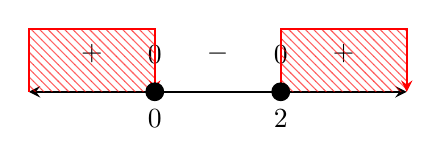
\begin{tikzpicture}[scale=0.8]
\draw[thick,stealth-stealth] (-2,0)--(4,0);
\node[above] at (-1,0.3) {$+$};
\node[above] at (0,0.3) {$0$};
\node[above] at (1,0.3) {$-$};
\node[above] at (2,0.3) {$0$};
\node[above] at (3,0.3) {$+$};
\draw[thick,-stealth,Red] (-2,0)--(-2,1)--(0,1)--(0,0);
\draw[thick,-stealth,Red] (2,0)--(2,1)--(4,1)--(4,0);
\path[pattern=north west lines,opacity=.6,pattern color=Red] (-2,0)--(-2,1)--(0,1)--(0,0)--cycle;
\path[pattern=north west lines,opacity=.6,pattern color=Red] (2,0)--(2,1)--(4,1)--(4,0)--cycle;
\filldraw[black,fill=black] (0,0) node[below,yshift=-.1cm] {$0$} circle (0.4em);
\filldraw[black,fill=black] (2,0) node[below,yshift=-.1cm] {$2$} circle (0.4em);
\end{tikzpicture} &
20 & \\
\midrule
\multicolumn{2}{r}{\textbf{Jumlah}} & 100 & \\
\end{rubrik}

\butir{Butir 3. $\displaystyle \left|\frac{2-3x}{x+3}\right| \geq \frac{1}{4}$ (100 poin)}
\begin{rubrik}
Langkah &
Satu sifat nilai mutlak, titik kritis termasuk $x = -3$, lalu analisis tanda. &
50 & \\
Jawaban &
$\mathrm{HP} = (-\infty, -3) \cup \bigl(-3, \frac{5}{13}\bigr] \cup [1, \infty)$. &
30 & \\
Penyajian &
Garis bilangan: $x = -3$ terbuka, titik $\frac{5}{13}$ dan $1$ penuh.\par\vspace{0.4em}
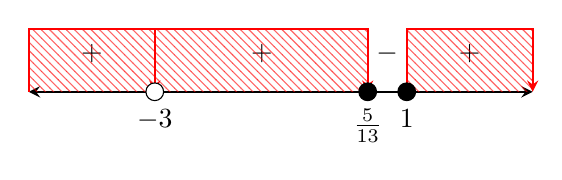
\begin{tikzpicture}[scale=0.8]
\draw[thick,stealth-stealth] (-5,0)--(3,0);
\node[above] at (-4,0.3) {$+$};
\node[above] at (-1.3,0.3) {$+$};
\node[above] at (0.69,0.3) {$-$};
\node[above] at (2,0.3) {$+$};
\draw[thick,-stealth,Red] (-5,0)--(-5,1)--(-3,1)--(-3,0);
\draw[thick,-stealth,Red] (-3,0)--(-3,1)--(0.38,1)--(0.38,0);
\draw[thick,-stealth,Red] (1,0)--(1,1)--(3,1)--(3,0);
\path[pattern=north west lines,opacity=.6,pattern color=Red] (-5,0)--(-5,1)--(-3,1)--(-3,0)--cycle;
\path[pattern=north west lines,opacity=.6,pattern color=Red] (-3,0)--(-3,1)--(0.38,1)--(0.38,0)--cycle;
\path[pattern=north west lines,opacity=.6,pattern color=Red] (1,0)--(1,1)--(3,1)--(3,0)--cycle;
\filldraw[black,fill=black] (0.38,0) node[below,yshift=-.1cm] {$\frac{5}{13}$} circle (0.4em);
\filldraw[black,fill=black] (1,0) node[below,yshift=-.1cm] {$1$} circle (0.4em);
\filldraw[black,fill=white] (-3,0) node[below,yshift=-.1cm] {$-3$} circle (0.4em);
\end{tikzpicture} &
20 & \\
\midrule
\multicolumn{2}{r}{\textbf{Jumlah}} & 100 & \\
\end{rubrik}

\butir{Butir 4. $\displaystyle \left|\frac{2x}{7} - 5\right| \geq 7$ (100 poin)}
\begin{rubrik}
Langkah &
Satu sifat $|u| \geq a$ (dua kasus) atau sifat lain yang setara, sampai kedua batas diperoleh. &
50 & \\
Jawaban &
$\mathrm{HP} = (-\infty, -7] \cup [42, \infty)$. &
30 & \\
Penyajian &
Garis bilangan: titik penuh di $-7$ dan $42$, arsiran ke luar.\par\vspace{0.4em}
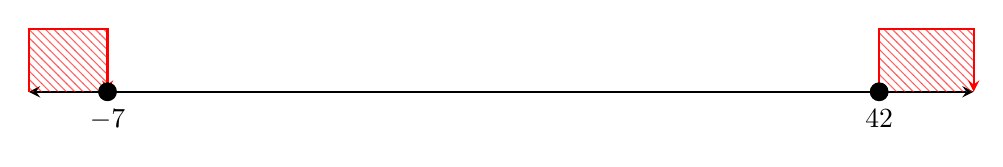
\begin{tikzpicture}[scale=0.8]
\draw[thick,stealth-stealth] (-3,0)--(12,0);
\draw[thick,-stealth,Red] (-3,0)--(-3,1)--(-1.75,1)--(-1.75,0);
\draw[thick,-stealth,Red] (10.5,0)--(10.5,1)--(12,1)--(12,0);
\path[pattern=north west lines,opacity=.6,pattern color=Red] (-3,0)--(-3,1)--(-1.75,1)--(-1.75,0)--cycle;
\path[pattern=north west lines,opacity=.6,pattern color=Red] (10.5,0)--(10.5,1)--(12,1)--(12,0)--cycle;
\filldraw[black,fill=black] (-1.75,0) node[below,yshift=-.1cm] {$-7$} circle (0.4em);
\filldraw[black,fill=black] (10.5,0) node[below,yshift=-.1cm] {$42$} circle (0.4em);
\end{tikzpicture} &
20 & \\
\midrule
\multicolumn{2}{r}{\textbf{Jumlah}} & 100 & \\
\end{rubrik}

\butir{Butir 5. $\displaystyle \left|\frac{x-1}{3x+1}\right| \leq \frac{7}{2}$ (100 poin)}
\begin{rubrik}
Langkah &
Satu sifat nilai mutlak, titik kritis termasuk $x = -\frac{1}{3}$, lalu irisan atau analisis tanda. &
50 & \\
Jawaban &
$\mathrm{HP} = \bigl(-\infty, -\frac{9}{19}\bigr] \cup \bigl[-\frac{5}{23}, \infty\bigr)$, dengan $x = -\frac{1}{3}$ tidak masuk. &
30 & \\
Penyajian &
Garis bilangan sesuai HP: penuh di $-\frac{9}{19}$ dan $-\frac{5}{23}$, lubang di $-\frac{1}{3}$.\par\vspace{0.4em}
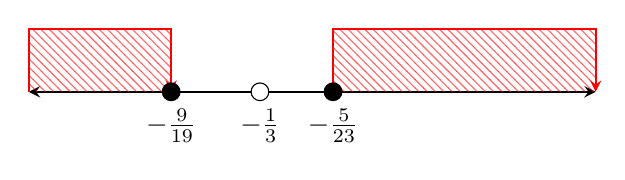
\begin{tikzpicture}[scale=0.8]
\draw[thick,stealth-stealth] (-7,0)--(2,0);
\draw[thick,-stealth,Red] (-7,0)--(-7,1)--(-4.74,1)--(-4.74,0);
\draw[thick,-stealth,Red] (-2.17,0)--(-2.17,1)--(2,1)--(2,0);
\path[pattern=north west lines,opacity=.6,pattern color=Red] (-7,0)--(-7,1)--(-4.74,1)--(-4.74,0)--cycle;
\path[pattern=north west lines,opacity=.6,pattern color=Red] (-2.17,0)--(-2.17,1)--(2,1)--(2,0)--cycle;
\filldraw[black,fill=black] (-4.74,0) node[below,yshift=-.1cm] {$-\frac{9}{19}$} circle (0.4em);
\filldraw[black,fill=white] (-3.33,0) node[below,yshift=-.1cm] {$-\frac{1}{3}$} circle (0.4em);
\filldraw[black,fill=black] (-2.17,0) node[below,yshift=-.1cm] {$-\frac{5}{23}$} circle (0.4em);
\end{tikzpicture} &
20 & \\
\midrule
\multicolumn{2}{r}{\textbf{Jumlah}} & 100 & \\
\end{rubrik}

\section*{Rekap skor}
\noindent
\begin{tabular}{@{}lr@{}}
\toprule
Butir & Skor \\
\midrule
1 & \\
2 & \\
3 & \\
4 & \\
5 & \\
\midrule
Rata-rata = jumlah skor / 5 (maksimum 100) & \\
\bottomrule
\end{tabular}

\end{document}
